% !TEX root = ../pdf/lsj.tex
% [There are multiple lsj.tex files, but the one in ../pdf is the usual one]


%%%%%%%%%%%%%%%%%%%%%%%%%%%%%%%%%%%%%%%%%%%%%%%
\chapter{Getting started with JASP\label{ch:introj}}

\begin{quote}
{\it Robots are nice to work with.}\\ 
\hspace*{2cm}--Roger Zelazny\FOOTNOTE{Source: {\it Dismal Light} (1968).}
\end{quote}


\noindent
In this chapter we'll discuss how to get started in JASP. We'll briefly talk about how to download and install JASP, but most of the chapter will be focused on getting you started with finding your way around the JASP user interface. Our goal in this chapter is \emph{not} to learn any statistical concepts: instead, we're just trying to learn the basics of how JASP works and get comfortable interacting with the system. To do this we'll spend some time looking at datasets and variables. In doing so, you'll get a bit of a feel for what it's like to work in JASP. 

However, before going into any of the specifics, it's worth talking a little about why you might want to use JASP at all. Given that you're reading this you've probably got your own reasons. However, if those reasons are ``because that's what my stats class uses'', it might be worth explaining a little why your professor has chosen to use JASP for the class. Of course, who really knows why {\it other} people choose JASP, so really, I will be talking about why I use it.
\begin{itemize}
\item It's sort of obvious but worth saying anyway: doing statistics on a computer is faster, easier and more powerful than doing statistics by hand. Computers excel at mindless repetitive tasks, and a lot of statistical calculations are both mindless and repetitive. For most people the only reason to ever do statistical calculations with pencil and paper is for learning purposes (even professionals do this when learning new concepts). In my class I do occasionally suggest doing some calculations that way, but the only real value to it is pedagogical. It does help you to get a ``feel'' for statistics to do some calculations yourself, so it's worth doing it once. But only once!
\item Doing statistics in a conventional spreadsheet (e.g., Microsoft Excel) is generally a bad idea in the long run. Although many people likely feel more familiar with them, spreadsheets are very limited in terms of what analyses they allow you do. If you get into the habit of trying to do your real life data analysis using spreadsheets then you've dug yourself into a very deep hole.
\item Avoiding proprietary software is a very good idea. There are a lot of commercial packages out there that you can buy, some of which I like and some of which I don't. They're usually very glossy in their appearance and generally very powerful (much more powerful than spreadsheets). However, they're also very expensive. Usually, the company sells ``student versions'' (crippled versions of the real thing) very cheaply, and then they they sell full powered ``educational versions'' at a price that makes me wince. They will also sell commercial licences with a staggeringly high price tag. The business model here is to suck you in during your student days and then leave you dependent on their tools when you go out into the real world. It's hard to blame them for trying, but personally I'm not in favor of shelling out thousands of dollars if I can avoid it. And you can avoid it. If you make use of packages like JASP that are open source and free you never get trapped having to pay exorbitant licensing fees. 
\end{itemize}
Those are the main reasons I use JASP. It's not without its flaws, though. It's relatively new\FOOTNOTE{As of writing this in May 2019.} so there is not a huge set of textbooks and other resources to support it, and it has a few annoying quirks that we're all pretty much stuck with, but on the whole I think the strengths outweigh the weakness; more so than any other option I've encountered so far. 


\section{Installing JASP \label{sec:gettingjasp}}

Okay, enough with the sales pitch. Let's get started. Just as with any piece of software, JASP needs to be installed on a computer. Fortunately, JASP is freely distributed online and you can download it from the JASP homepage, which is:
\begin{quote}
\url{https://jasp-stats.org/}
\end{quote}
At the top of the page, you'll click on the heading ``Download''. Then, you'll see separate links for Windows users, Mac users, and Linux users. If you follow the relevant link you'll see that the online instructions are pretty self-explanatory. As of this writing, the current version of JASP is 0.9.2.0, but they usually issue updates every few months, so you'll probably have a newer version.\FOOTNOTE{Although JASP is updated frequently it doesn't usually make much of a difference for the sort of work we'll do in this book. In fact, during the writing of the book I upgraded several times and it didn't make much difference at all to what is in this book.}

\SUBSECTION{Starting up JASP}

One way or another, regardless of what operating system you're using, it's time to open JASP and get started. When first starting JASP you will be presented with a user interface which looks something like Figure \ref{fig:startingjasp}.

\begin{figure}[ht]
\begin{center}
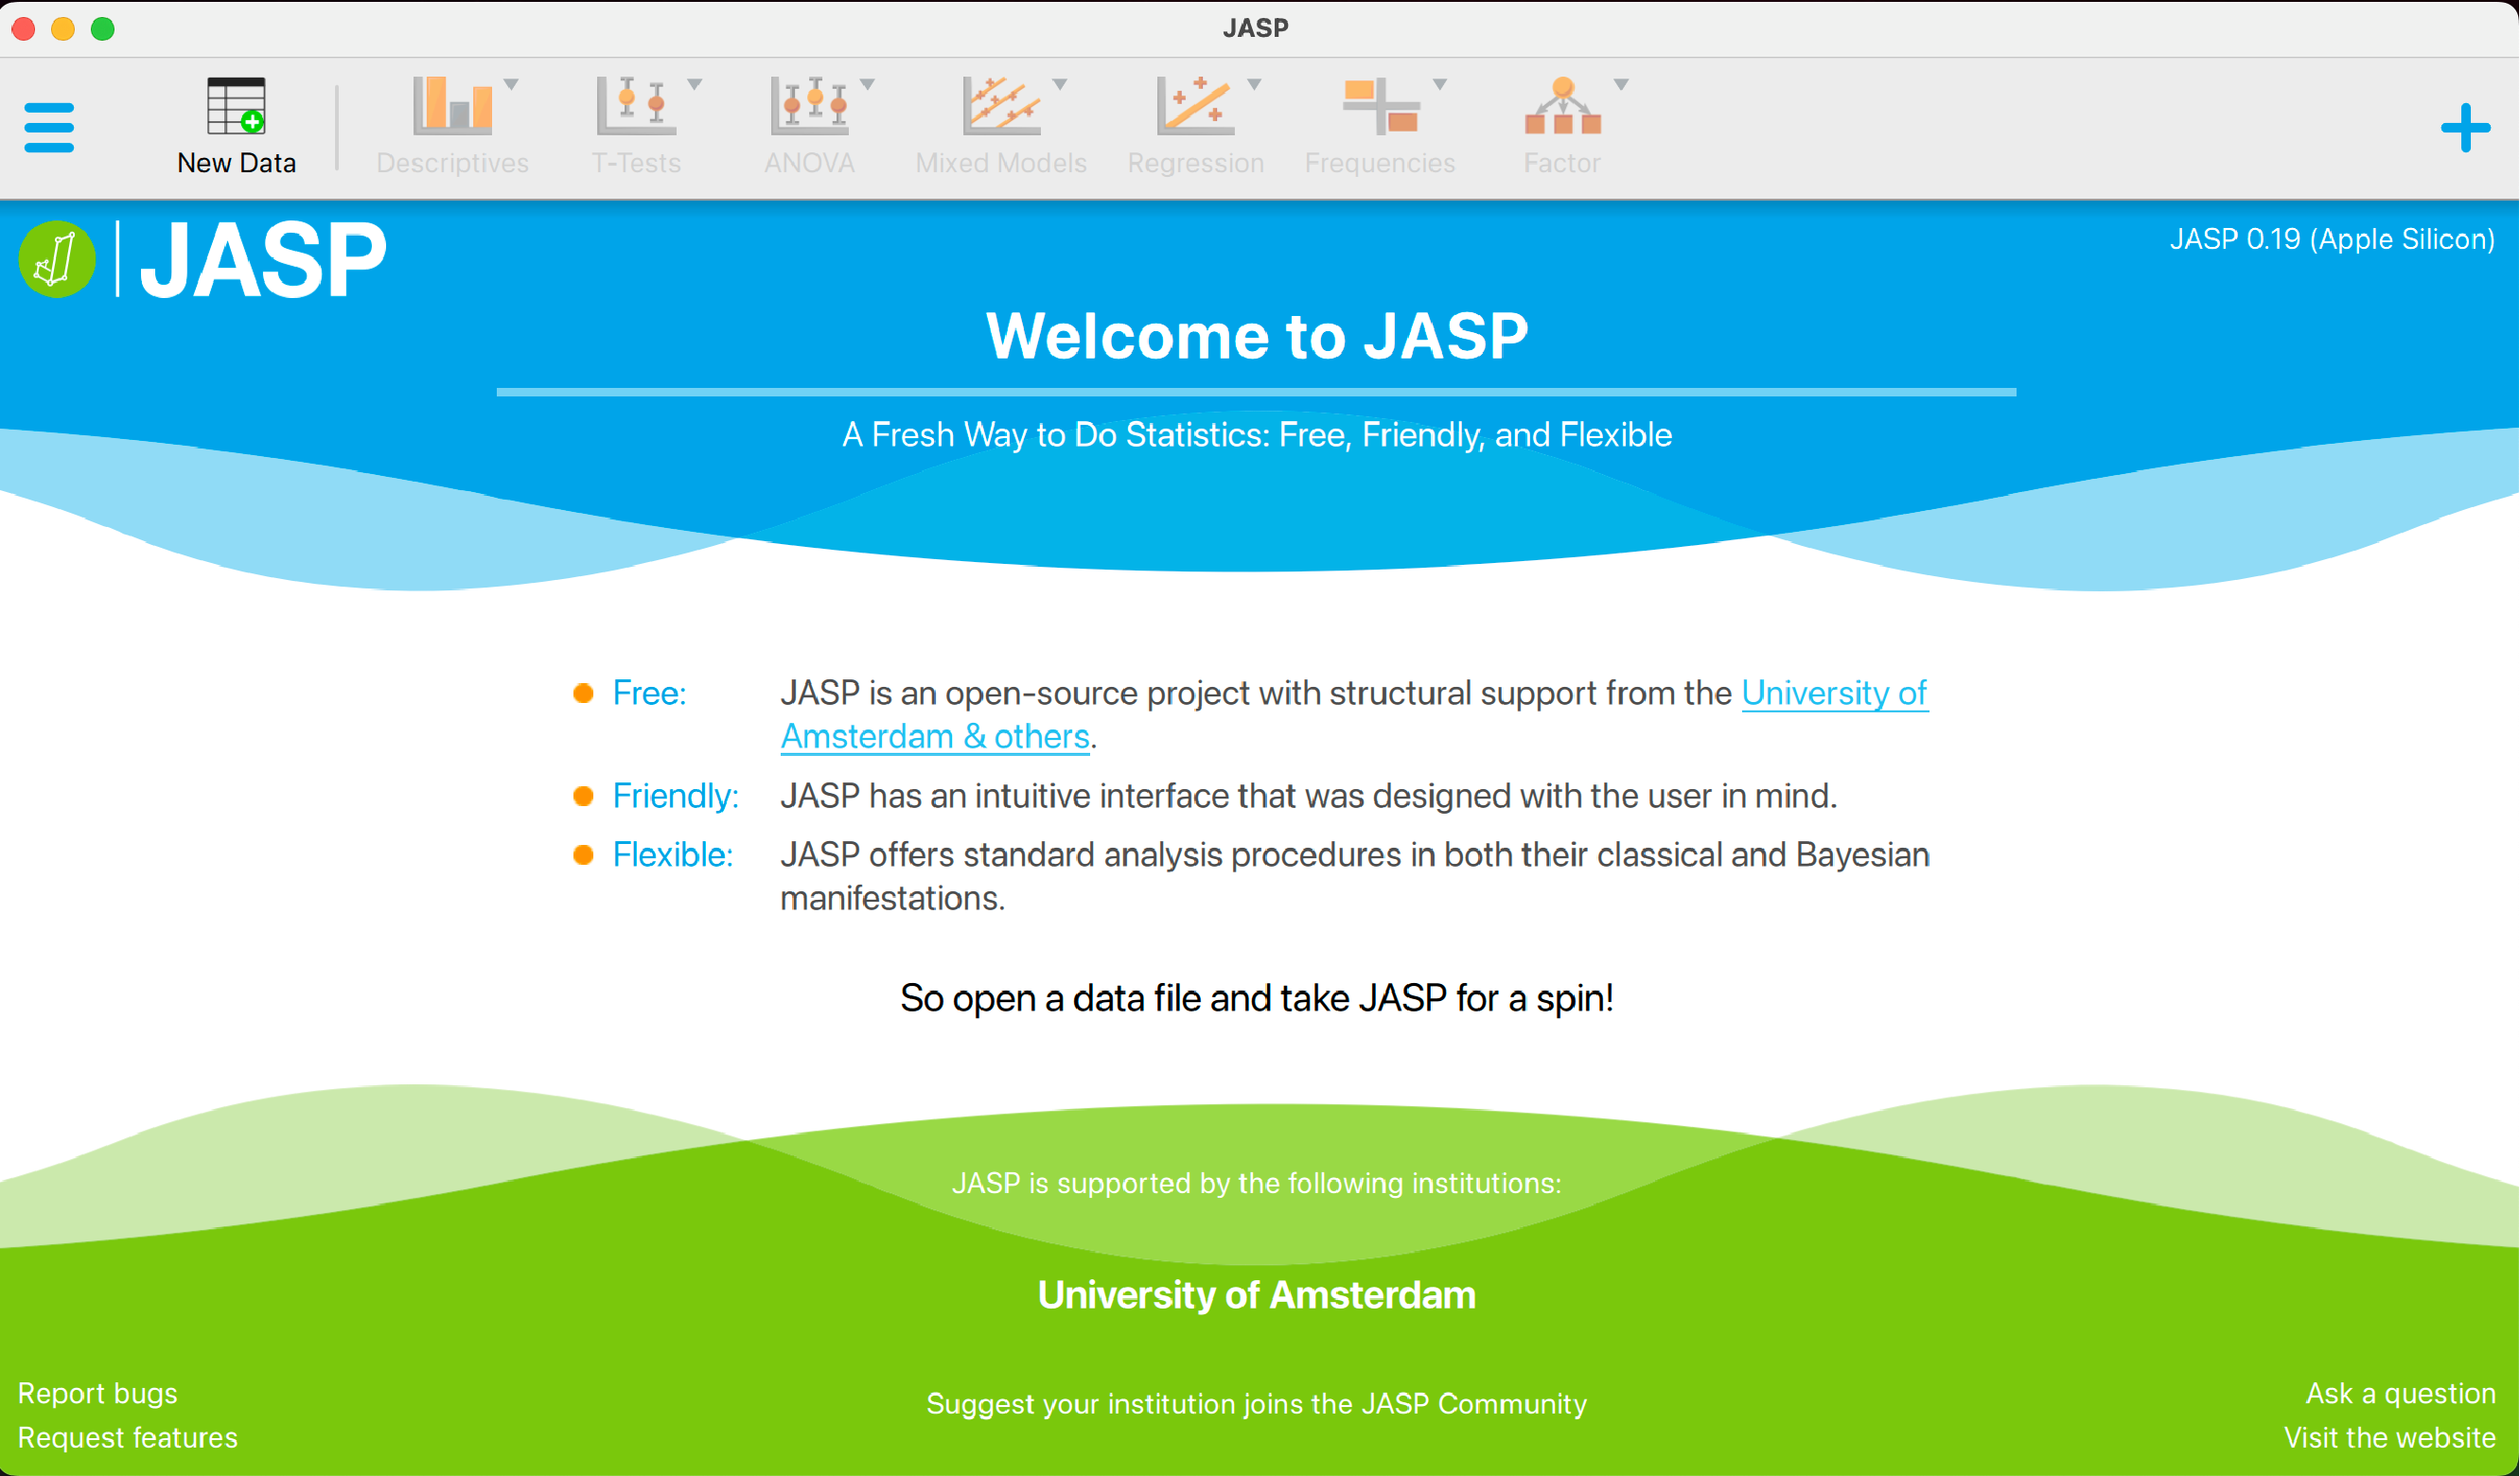
\includegraphics[width=14cm]{../img/introj/startingjasp.pdf}
\caption{JASP looks like this when you start it.}
%\HR
\label{fig:startingjasp}
\end{center}
\end{figure}

If you have experience with other statistical software packages, you might be a bit dismayed to see that there is no place to begin typing your data. This is a deliberate decision on the part of the JASP developers; their philosophy is that users should be allowed to use the editor they are most comfortable with \FOOTNOTE{See https://jasp-stats.org/2018/05/15/data-editing-in-jasp/ for a discussion of this very issue.}. Thus, the preferred method for getting data into JASP is to load a CSV file (.csv), which is a text-based data format that can be created by (and opened in) any spreadsheet program. More details about this will be given shortly. 

\section{Analyses\label{sec:analyses}}

Analyses can be selected from several buttons along the top. Selecting an analysis will present an ‘options panel’ for that particular analysis, allowing you to assign different variables to different parts of the analysis, and select different options. At the same time, the results for the analysis will appear in the right ‘Results panel’ and will update in real-time as you make changes to the options.

When you have the analysis set up correctly you can dismiss the analysis options by clicking the 'OK' button in the top right of the optional panel. If you wish to return to these options, you can click on the results that were produced. In this way, you can return to any analysis that you (or say, a colleague) created earlier.

If you decide you no longer need a particular analysis, you can remove it with the results context menu. Clicking on the header of a specific results header (or clicking on the $\blacktriangledown$ symbol) will bring up a menu and by selecting ‘Remove Analysis’, the analysis can be removed. But more on this later. First, let's get some data into JASP. %take a more detailed look at the spreadsheet view.

\section{Loading data in JASP\label{sec:load}}

There are several different types of files that are likely to be relevant to us when doing data analysis. There are two in particular that are especially important from the perspective of this book:
\begin{itemize}
\item {\it .jasp files} are those with a \filename{.jasp} file extension. This is the standard kind of file that JASP uses to store data, and variables and analyses. 
\item {\it Comma separated value (CSV) files} are those with a \filename{.csv} file extension. These are just regular old text files and they can be opened with many different software programs. It's quite typical for people to store data in csv files, precisely because they're so simple.
\end{itemize} 


\SUBSECTION{Importing data from CSV files}

One quite commonly used data format is the humble ``comma separated value'' file, also called a CSV file, and usually bearing the file extension \filename{.csv}. CSV files are just plain old-fashioned text files and what they store is basically just a table of data. This is illustrated in Figure~\ref{fig:booksalescsv}, which shows a file called \filename{booksales.csv} that I've created. As you can see, each row represents the book sales data for one month. The first row doesn't contain actual data though, it has the names of the variables.

\begin{figure}
\begin{center}
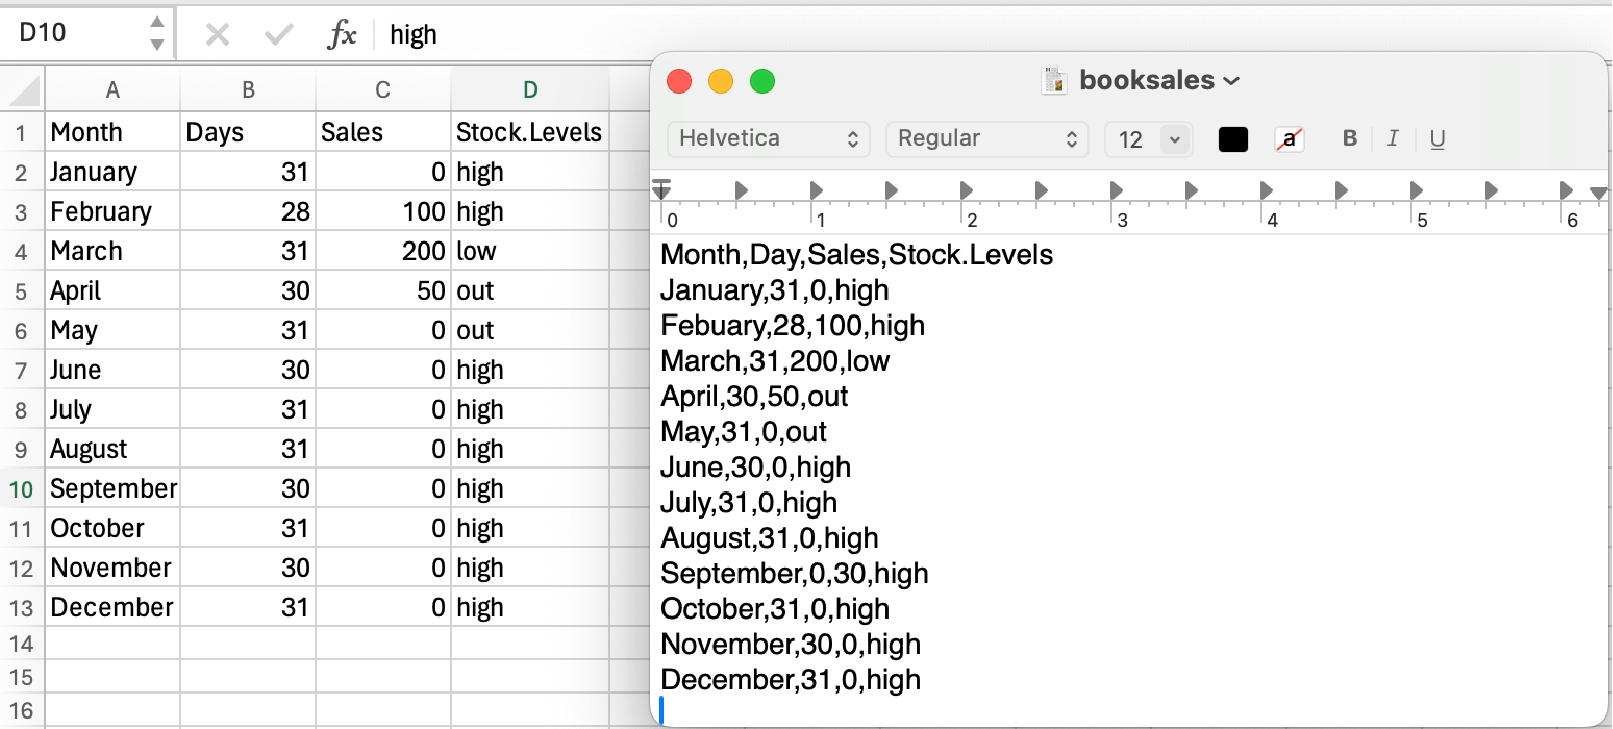
\includegraphics[width=14cm]{../img/introj/booksalescsv.pdf}
\caption{The \filename{booksales.csv} data file. On the left I've opened the file using a spreadsheet program, which shows that the file is basically a table. On the right the same file is open in a standard text editor (the TextEdit program on a Mac), which shows how the file is formatted. The entries in the table are separated by commas.}
\HR
\label{fig:booksalescsv}
\end{center}
\end{figure} 

Once you have a CSV file (either that you created or someone has given you), you open the file in JASP by clicking the File tab at the top left hand corner, select ‘Open’, and then choosing from the options presented. Most commonly, you will select 'Computer' and then 'Browse', which will then open a file browser specific to your operating system.  If you're on a Mac, it'll look like the usual Finder window that you use to choose a file; on Windows it looks like an Explorer window. An example of what it looks like on a Mac is shown in Figure~\ref{fig:fileopen}. I'm assuming that you're familiar with your own computer, so you should have no problem finding the csv file that you want to import! Find the one you want, then click on the ``Open'' button. 

\begin{figure}[t]
\begin{center}
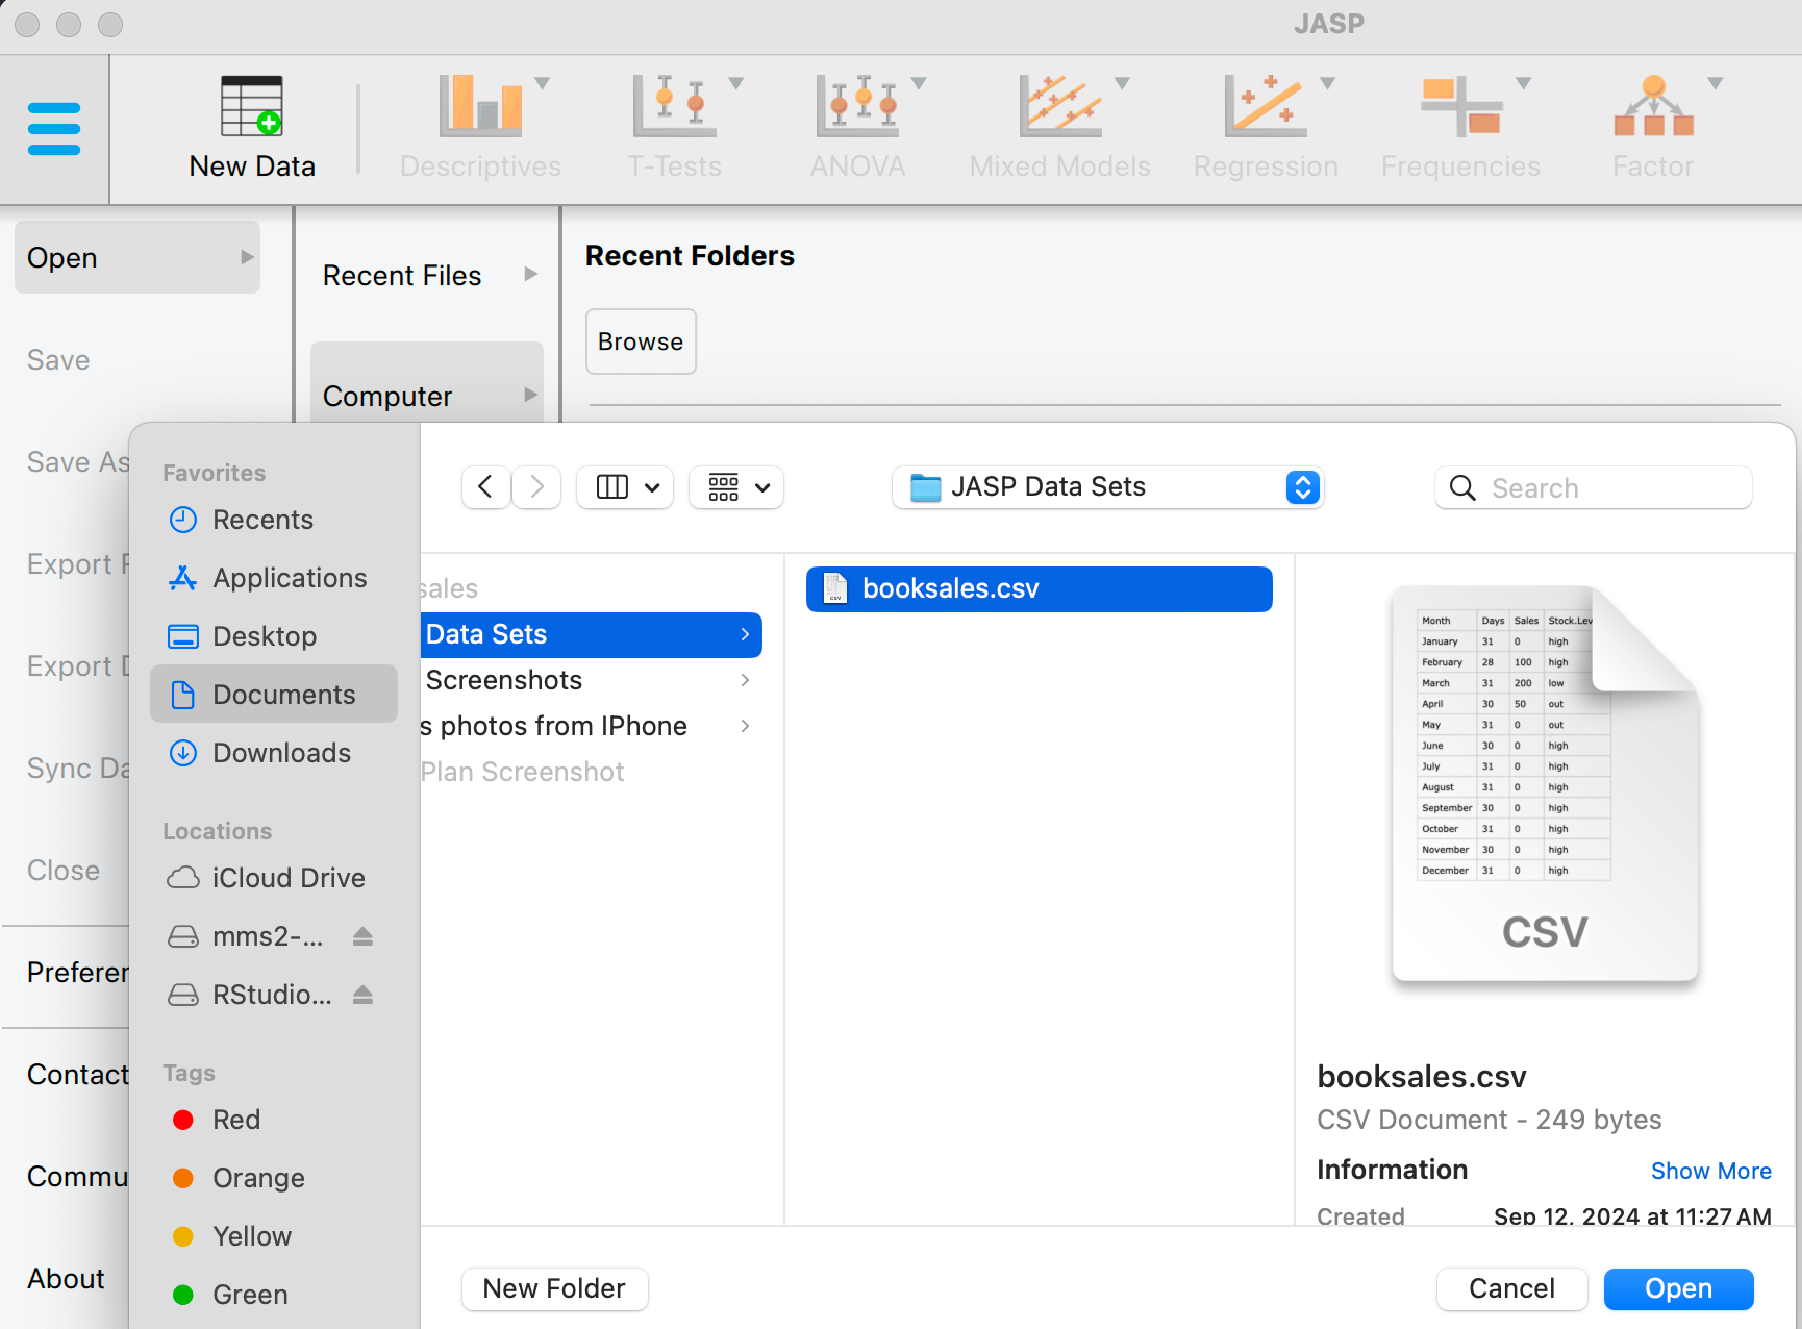
\includegraphics[width=14cm]{../img/introj/openscreen.pdf}
\caption{A dialog box on a Mac asking you to select the CSV file JASP should try to import. Mac users will recognise this immediately -- it's the usual way in which a Mac asks you to find a file. Windows users won't see this, but instead will see the usual explorer window that Windows always gives you when it wants you to select a file.}
\HR
\label{fig:fileopen}
\end{center}
\end{figure} 

\section{The spreadsheet\label{sec:spreadsheet}}

Once loaded into JASP, data is represented in a spreadsheet with each column representing a ‘variable’ and each row representing a ‘case’ or ‘participant’.

\SUBSECTION{Variables}

The most commonly used variables in JASP are ‘Data Variables’, which contain data loaded from a CSV file. Data variables can be one of three measurement levels, which are designated by the symbol in the header of the variable’s column.

{\it Nominal} variables are for categorical variables which are text labels, for example a column called Gender with the values Male and Female would be nominal. So would a person’s name. Nominal variable values can also have a numeric value. These variables are used most often when importing data which codes values with numbers rather than text. For example, a column in a dataset may contain the values 1 for males, and 2 for females. It is possible to add nice ‘human-readable’ labels to these values with the variable editor (more on this later).

{\it Ordinal} variables are like Nominal variables, except the values have a specific order. An example is a Likert scale with 3 being ‘strongly agree’ and -3 being ‘strongly disagree’.

{\it Scale} variables are variables which exist on a continuous scale. Examples might be height or weight. This is also referred to as ‘Interval’ or ‘Ratio scale’.

Note that when opening a data file JASP will try and guess the variable type from the data in each column. In both cases this automatic approach may not be correct, and it may be necessary to manually specify the variable type with the variable editor.

\SUBSECTION{Computed variables}

Computed Variables are those which take their value by performing a computation on other variables. Computed Variables can be used for a range of purposes, including log transforms, z-scores, sum-scores, negative scoring and means.

Computed variables can be added to the data set with the ‘+’ button in the header row of the data spreadsheet. This will produce a dialog box where you can specify the formula using either R code or a drag-and-drop interface. At this point, I simply want you to know that the capability exists, but describing how to do it is a little beyond our scope right now.  More later!

\SUBSECTION{Copy and Paste\label{sec:copypaste}}

As a final note, we will mention that JASP produces nice American Psychological Association (APA) formatted tables and attractive plots. It is often useful to be able to copy and paste these, perhaps into a Word document, or into an email to a colleague. To copy results, click on the header of the object of interest and from the menu select exactly what you want to copy. Selecting ``copy'' copies the content to the clipboard and this can be pasted into other programs in the usual way. You can practice this later on when we do some analyses. Also, if you use the \LaTeX document preparation system, you can select ``Copy special'' and ``LaTeX code''; doing so will place the \LaTeX syntax into your clipboard.


\section{Changing data from one measurement scale to another\label{sec:coercion}}

Sometimes you want to change the variable level. This can happen for all sorts of reasons. Sometimes when you import data from files, it can come to you in the wrong format. Numbers sometimes get imported as nominal, text values. Dates may get imported as text. ParticipantID values can sometimes be read as continuous: nominal values can sometimes be read as ordinal or even continuous. There's a good chance that sometimes you'll want to convert a variable from one measurement level into another one. Or, to use the correct term, you want to \keyterm{coerce} the variable from one class into another. 

In \ref{sec:spreadsheet} we saw how to specify different variable levels, and if you want to change a variable's measurement level then you can do this in the JASP data view for that variable. Just click the check box for the measurement level you want - continuous, ordinal, or nominal. 


\section{Quitting JASP \label{sec:quittingjasp}}

There's one last thing I should cover in this chapter: how to quit JASP. It's not hard, just close the program the same way you would any other program. However, what you might want to do before you quit is save your work! There are two parts to this: saving any changes to the data set, and saving the analyses that you ran.

It is good practice to save any changes to the data set as a {\it new} data set. That way you can always go back to the original data. To save any changes in JASP, select `Export Data' from the `File' tab, click 'Browse' and navigate to the directory location in which you want to save the file, and create a new file name for the changed data set.

Alternatively, you can save {\it both} the changed data and any analyses you have undertaken by saving as a \filename{.jasp} file. To do this, from the 'File' tab select `Save as', click 'Browse' to navigate to the directory location in which you want to save the file, and type in a file name for this \filename{.jasp} file. Remember to save the file in a location where you can find it again later. I usually create a new folder for specific data sets and analyses.  


\section{Summary}

Every book that tries to teach a new statistical software program to novices has to cover roughly the same topics, and in roughly the same order. Ours is no exception, and so in the grand tradition of doing it just the same way everyone else did it, this chapter covered the following topics:

\begin{itemize}
\item Section~\ref{sec:gettingjasp}. We downloaded and installed JASP, and started it up.
\item Section~\ref{sec:analyses}. We very briefly oriented to the part of JASP where analyses are done and results appear, but then deferred this until later in the book.
\item Section~\ref{sec:load}. We saw how to load data files (formatted as \filename{.csv} files) in JASP.
\item Section~\ref{sec:spreadsheet}. We spent more time looking at the spreadsheet part of JASP, and considered different variable types, and briefly mentioned how to compute new variables.
\item Section~\ref{sec:coercion}. And saw that sometimes we need to coerce data from one type to another.
\item Section~\ref{sec:quittingjasp}. Finally, we looked at good practice in terms of saving your data set and analyses when you have finished and are about to quit JASP.
\end{itemize}

\noindent
We still haven't arrived at anything that resembles data analysis. Maybe the next chapter will get us a bit closer!



